% chap2.tex (Definitions)

\chapter{Literature Review}\label{Literature Review}

A tree-based method (or recursive partitioning) divides data recursively to attain multiple mutually exclusive sub-groups. Tree-based methods are very effective in handling multifaceted data and acquiring acknowledgment as a sound technique for addressing data complexity, which renders them attractive in different application fields. The proposal of Classification and Regression Tree (CART) \citep{breiman1984classification} made the tree models more popular and widely accepted in applications and the current norm of tree modeling. %\cite{loh2011classification} stated that the classification and regression tree methods obtain their models through the recursive partitioning of the datasets, fitting a simple model within each partition and these partitionings can be represented graphically as a decision tree. 

\section{Decision Trees}
A decision tree is a graphical representation of specific decision situations that are used when complex branching occurs in a structured decision \citep{njoku2019decision}. While in data mining a decision tree is a predictive model which can be used to represent both classifiers and regression models, in operations research decision trees refer to a hierarchical model of decisions and their consequences \citep{maimon2014data}. The implementation of decision trees originated from decision theory and statistics. One of the best and most applied supervised learning algorithm in predictive modeling is decision trees which also works in connection with ensemble methods for more accurate results. Decision trees are general purpose prediction and classification mechanisms that were among the first statistical algorithms to be implemented in electronic form during the adoption of digital circuitry to electronic computations in the latter decades of the 20th century \citep{de2013decision}. According to \cite{hu2019optimal}, Decision trees are one of the leading forms of interpretable models and despite several attempts over the last several decades to improve the optimality of decision tree algorithms, the CART \citep{breiman1984classification} and C4.5 \citep{quinlan1993program} decision tree algorithms (and other greedy tree-growing variants) have remained as dominant methods in practice. Obtaining a decision tree model according to the CART \citep{breiman1984classification} convention involves growing a large initial tree, a pruning algorithm for reducing the tree size, and a validation method for determining the best tree. Tree methods are also an excellent tool for grouping. Once a final tree structure is obtained, the groups are naturally induced by its terminal nodes.

The decision tree consists of three types of nodes that are a root node that has no incoming edge, an internal or test node that has exactly one incoming edge, and outgoing edges and leaves (terminal or decision nodes). According to a given function of the input attributes values, each internal node splits an instance space into two or more sub-spaces on a decision tree. 

\begin{figure}[H]
%	\begin{tiny}
	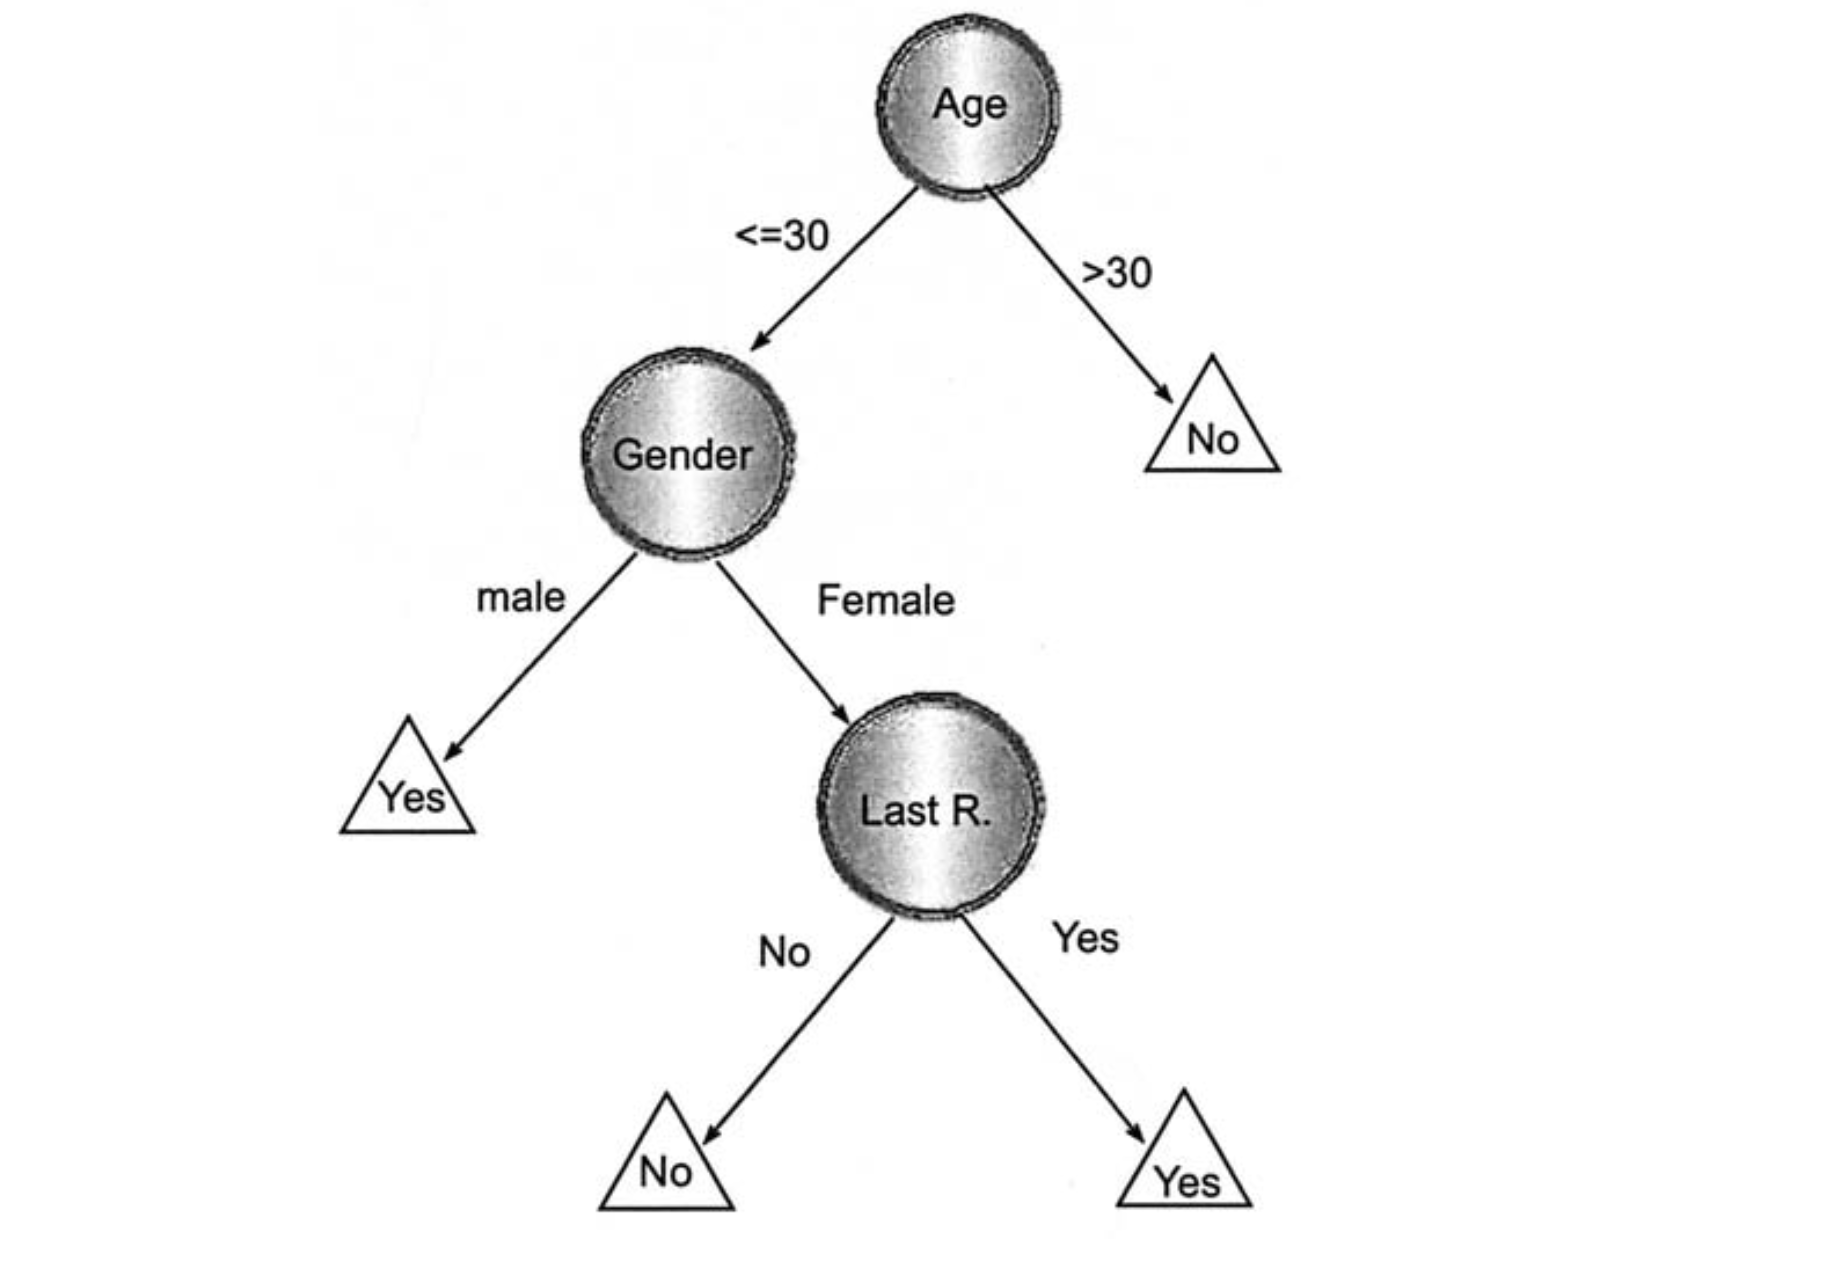
\includegraphics[width=\linewidth]{tree.png}
	\caption{Decision tree presenting response to direct mailing. Sourced from \emph{Decision trees in Data mining and knowledge discovery handbook} (pages 165–192), by Rokach, L. and Maimon, O. (2005) Springer.}
	\label{trep}
	\centering
%\end{tiny}
\end{figure}

Figure \ref{trep} presents a decision tree that shows whether or not a potential customer will respond to a direct mailing. %The internal nodes are represented as circles, whereas leaves are denoted as triangles also each node is labeled with the attribute it tests, and its branches are labeled with its corresponding values.
Given Figure \ref{trep}, one can predict the response of a potential customer by sorting it down the tree and understand the behavioral characteristics of the entire potential customers population regarding direct mailing \citep{rokach2005decision}.


\section{Types of Decision Trees}
There are basically two types of trees;
\begin{itemize}
	\item Regression trees when the outcome or response variable is continuous, for example determing the price of a newly manufactured product by considering the various inputs and contraints.

	\item Classification trees (also known as decision trees) when the outcome is binary or categorical. A classical example is a toss of a coin which has only two outcomes whether a head or tail.
\end{itemize}	
 From a statistical perspective, regression as a whole is a broader concept that incorporates the classification problem as a special case.


\section{Extension of Decision Trees  and Recent development}
Decision trees as originally coined from tree models have undergone several recent developments. Oblique decision trees according to \cite{murthy1995growing} produce polygonal (polyhedral) partitionings of the attribute space, while conventional axis-parallel trees produce partitionings in the form of hyper-rectangles that are parallel to the feature axes. A general-purpose data structure for addressing the behaviors of recursive programs that interact with their surroundings is known as interaction trees (ITrees) \citep{xia2019interaction}. Interaction trees (ITrees) were employed by  \cite{su2008interaction} in their article, where ITrees was to optimize a subgroup analysis in comparative studies. Specifically, the IT method recursively partitions the data into two subsets that show the greatest interaction with the treatment, which results in a number of objectively defined subgroups \citep{su2008interaction}.

Decision trees have as well generated several extensions. Noticeable amongst them are Multivariate Adaptive Regression Splines (MARS), Hierarchical Mixture Model (HMM), and the Ensemble Methods (EM). Multivariate Adaptive Regression Splines (MARS) \citep{friedman1991multivariate} is a new method presented for flexible regression modeling of high dimensional data and this procedure is motivated by the recursive partitioning approach to regression and shares its attractive properties. While CART does piecewise constant modeling, MARS fits piecewise linear models. Also, \cite{jordan1994hierarchical} presented a tree-structured architecture for supervised learning and the statistical model underlying the architecture is a hierarchical mixture model in which both the mixture coefficients and the mixture components are generalized linear models (GLIM’s). Ensemble methods are machine learning technique that produces one optimal predictive model by combining usually hundreds or thousands base learners. By considering one decision tree and guessing to make the right decision at each split, ensemble methods make provision to take into consideration a sample of decision trees, evaluate which characteristics to employ or questions to enumerate at each split, and then make a final prediction as a result of the aggregated results of the sampled decision trees. Noticeable ensemble methods used in obtaining an optimal outcome in decision trees are Boosting, Bagging and Random Forests(RF). Bagging is a method used to improve on unstable estimators or classifiers in a learning model. Specifically by generating multiple versions of the classifier and using these to get an aggregated classifier to obtain the new model  \citep{breiman1996bagging}. Boosting \citep{freund1996experiments} serves as a tool to significantly minimize the error of any learning algorithm that consistently generates classifiers that are better than guessing randomly. Random Forest (RF) is a combination of trees such that each tree depends on independently random sampled vector values of the same distribution \cite{breiman2001random}.


% \cite{breiman2001random} defined random forest (RF) as a combination of trees such that each tree depends on the values of a random vector sampled independently and with the same distribution for all trees in the forest.


%\subsection{MARS}
 %However, this method produces continuous models with continuous derivatives unlike recursive partitioning \citep{friedman1991multivariate}. Models that includes interactions in at most a few variables or relationships that are most likely additive can be flexibly and powerfully be modelled by this MARS approach \citep{friedman1991multivariate}.

%\subsection{Hierarchical Mixtures of Experts}
%An Expectation-Maximization (EM) algorithm for adjusting the parameters of the architecture was employed through maximum likelihood to learn the model \citep{jordan1994hierarchical}.

%\subsection{Ensemble Methods}

 
 
 %\begin{itemize}
 	
 %	\item\textbf{Bagging} is a method for generating multiple versions of a predictor and using these to get an aggregated predictor \citep{breiman1996bagging}. \cite{quinlan1996bagging} stated  that bagging requires that the learning system should not be stable so that small changes to the training set should lead to different classifiers.
 	
 %	\item \textbf{Boosting} is an accepted technique for enhancing the performance of any given learning algorithms. According to \citep{freund1996experiments}, in theory, boosting serves a tool to significantly minimize the error of any learning algorithm that consistently generates classifiers which need only be a bit better than guessing randomly. 
 	
 	
 %	\item \textbf{Random Forests (RF)} according  to \citep{breiman2001random} are a combination of tree predictors such that each tree depends on the values of a random vector sampled independently and with the same distribution for all trees in the forest. Random Forest is fast, robust to noise, does not overfit and offers possibilities for explanation and visualization of its output \citep{robnik2004improving}.
% \end{itemize}
 

%\section{Recent development}

\section{Problem with Inference}
One major difficulty in summarizing decision trees is that it does not allow for statistical inferences such as confidence interval or hypothesis testing for the true node mean $\mu_t$. A naive approach in making a node inference is therefore to construct a $(1-\alpha) \times 100\%$ confidence interval (CI) or perform a hypothesis test using the two stochastics components $\bar{y}_t$ and $s_t$ from the tree summary. This approach, however, leads to an over-optimism of the estimates or too narrow confidence intervals. An accurate or prudent way of making a valid inference within terminal nodes of decision trees has been a long-standing challenge for statisticians. Among few works that have been done to overcome this challenge, \cite{loh2018subgroups} proposed using the bootstrap calibration (BC) approach \citep{loh1987calibrating, loh1991bootstrap} to tune the confidence level. Particularly a best $\alpha'$ is sought such that $(1-\alpha')$ intervals of the same form as (\ref{eqn-naive-ci}) has the ($1-\alpha$) coverage for each terminal node.


